
% Define document class
\documentclass[twocolumn]{aastex631}

\newcommand{\flatiron}{\affiliation{Center for Computational Astrophysics, Flatiron Institute, New York, NY 10010, USA}}
% Begin!
\begin{document}

\title{Backpropagating Gravitational wave events}

\pacs{}

\author{Kaze W. K. Wong} 
\email{kwong@flatironinstitute.org}
\flatiron


\date{\today}

\begin{abstract}
In this
\end{abstract}

%\maketitle

\section{Introduction}

\begin{enumerate}
\item We have more and more event
\item Problem with population synthesis -> Need for developing algorithm to explore the high dimensional space
\item We run the event backward in time
\end{enumerate}

While forward modelling has been the canonical pathway to simulate binary systems and compare to GW observation,
it is not necessarily the most efficient way to constraint the underlying physical model.
Forward modelling of a binary system start with a set of initial binary parameters,
then evolve it until some stopping criteria is met,
typically either a merger event or the binary system stays stable for a Hubble time.
The problem is, most of the systems do not end in a merger, and the systems ending up as merger events do not necessarily agree with the observation.
This means if we want to evolve a binary to match the observation by pure trial and error, a large fraction of computation will be wasted in trying initial binary configurations that are not related to the observation.
To alleviate this inefficiency, the community often takes a population approach --- instead of trying to match binary systems to observations event by event,
one can draw systems from an initial population, forward model each member in that population then match it to the observed population properties.
However, this approach is essentially trading one inefficiency with another, since we still need to choose an initial distribution of binary parameters.
For relatively well-known source properties such as initial masses this is less of a problem,
but the distribution of some less well-studied properties such as common envelope efficiency is often heuristically chosen to be some simple distribution such as a delta function at some value, i.e. a fixed value for the entire population.
This is a problem when the target of a study is to understand these less studied parameters, since one either need to justify their choice of distribution,
or they should vary the family of distributions.

In this paper, instead of forward modelling the population of binary star to match observed GW events population,
we propose a method to "backward" model each GW event to its progenitor state.


This paper introduces a number of new perspectives in the study of binary evolution physics and gravitational-wave progenitors:
\begin{enumerate}
\item Instead of starting from a distribution 
\item Using derivative-based optimization algorithm, we are allowed to explore a moderate size parameter space 
\end{enumerate}

\section{Method}

We define the parameters that describe the progenitor's properties such as ZAMS masses and eccentricity as progenitor parameters $\bm{\theta'}$,
the parameters that control different physical prescriptions such as wind strength and common envelope efficiency as hyper-parameters $\bm{\lambda}$,
and random variables that affect certain stochastic process such as whether natal kick unbinds a binary as $\bm{X}$.
To avoid clutter in the following derivation,
we denote all the parameters related to mapping a particular progenitor system into a GW event collectively as evolutionary parameters $\bm{\Theta}$,
which includes $\bm{\theta'}$, $\bm{\lambda}$, and $\bm{X}$.

Once all the parameters including a particular draw of all the random variables are known,
the population synthesis code is a deterministic function that transforms the properties of the progenitors into the GW parameters.
Hence, the probability of obtaining a GW event with parameters $\bm{\theta}$ given the progenitor parameters $\bm{\theta}'$ is given by

\begin{align}
    p(\bm{\theta}|\bm{\Theta}) &= \bm{\delta}(\bm{f}(\bm{\Theta})-\bm{\theta}),
\end{align}

where $\bm{f}$ represents the population synthesis code.

While it is straightforward to write down the "forward" probability, the "backward" probability is more complicated since multiple evolutionary parameters can produce the same GW event.
Using Bayes theorem, the probability of an event with evolutionary parameters given the GW parameters can be derived as following

\begin{align}
    p(\bm{\Theta}|\bm{\theta}) &= \frac{p(\bm{\theta}|\bm{\Theta})p(\bm{\Theta})}{p(\bm{\theta})}, \nonumber \\
    &= \frac{p(\bm{\theta}|\bm{\Theta})p(\bm{\Theta})}{\int p(\bm{\theta}|\bm{\Theta}) p(\bm{\Theta}) d\bm{\Theta}}, \nonumber \\
    &= \frac{\bm{\delta}(\bm{f}(\bm{\Theta})-\bm{\theta})p(\bm{\Theta})}{\int d\bm{\theta} \bm{\delta}(f(\bm{\Theta})-\bm{\theta})p(\bm{\Theta})}.
\label{eq:backward_prob}
\end{align}

Using the result in eq.\ref{eq:backward_prob},
the probability of an event having evolutionary parameters given data can be obtained by marginalizing over the GW parameters

\begin{align}
    p(\bm{\Theta}|d) &= \int p(\bm{\Theta}|\bm{\theta}) p(\bm{\theta}|d) d\bm{\theta}\\
    &= \frac{1}{N}\sum_{i=1}^{N} p(\bm{\Theta}|\bm{\theta}_i). \label{eq:evolutionary_posterior}
\end{align}

The term $p(\bm{\theta}|d)$ is the inferred posterior probability for a particular event, which is usually presented by the LVK collaboration in the form of posterior samples.
In eq.\ref{eq:evolutionary_posterior}, we use importance sampling to turn the integration into a sum over the posterior samples.

For each posterior sample point, we can find the corresponding evolutionary parameters by solving an optimization problem that minimize the mean square difference between the GW event parameters and evolutionary parameters, i.e. 

\begin{align}
\mathcal{L}(\bm{\Theta},\bm{\theta}) = ||f(\bm{\Theta})-\bm{\theta}||^2
\label{eq:loss}
\end{align}

In principle, we should only accept solutions that exactly reproduce the LVK posterior samples.
However, it is not feasible to achieve such condition in practice, therefore we relax the condition in eq.\ref{eq:loss} to a small acceptance threshold, in our case we picked $10^{-2}$.
To make sure we find the complete set of progenitor parameters that corresponds to the posterior sample point, we use 1000 different initial guesses in solving the optimization problem.

Ideally we would like to have explicit control over all evolutionary parameters.
In particular, having explicit control over random variables allows us to marginalize over their contribution, so we can focus on progenitor parameters and hyper-parameters.
However, in practice most of the population synthesis simulation code (including \texttt{COSMIC} which we use in this study.) define their random variables implicitly,
i.e. the random variables are drawn within the program, instead of being arguments of the program.
This means the function we use to evolve the binary is not a deterministic function but a stochastic function instead. 
Hence, even if the root-finding algorithm performs perfectly,
forward modelling this set of roots does not guarantee to reproduce the set of posterior samples due to randomness of the evolution function.
To assure the recovered progenitor and hyper-parameters robustly corresponds to the posterior in the GW observables space,
we forward model ("Reproject) the recovered evolutionary parameters to the observables space to check whether the reprojected posterior agrees with the posterior given by the LVK collaboration.
We use KL divergence to measure the agreement between the two posterior distributions.
A small KL divergence means \texttt{COSMIC} is a viable channel for that specific event, otherwise it either means \texttt{COSMIC} can only explain part of the posterior or cannot explain the event at all.
This is completely expected since \texttt{COSMIC} comes with its own assumptions and is expected to fail in reproducing a subset of the event in GWTC3, such as event with at least one component beyond the pair instability supernova massgap.
On the other hand, the reprojection could subject to stochasticity in the evolution function we use.
Instead of reprojecting the posterior only once, we reproject the posterior multiple times with different random seeds and check whether the KL divergence varies significantly.
A varying KL divergence means this particular event is subjected to randomness in the evolution function, hence one should take extra caution in interpreting the result.


\section{Result}

\begin{enumerate}
\item Raw posterior of successful events.
\item Trace back the event's $z_{\rm ZAMS}$.
\item Reproject to observable space
\item Evidence ratio.
\end{enumerate}



% \begin{figure}
% 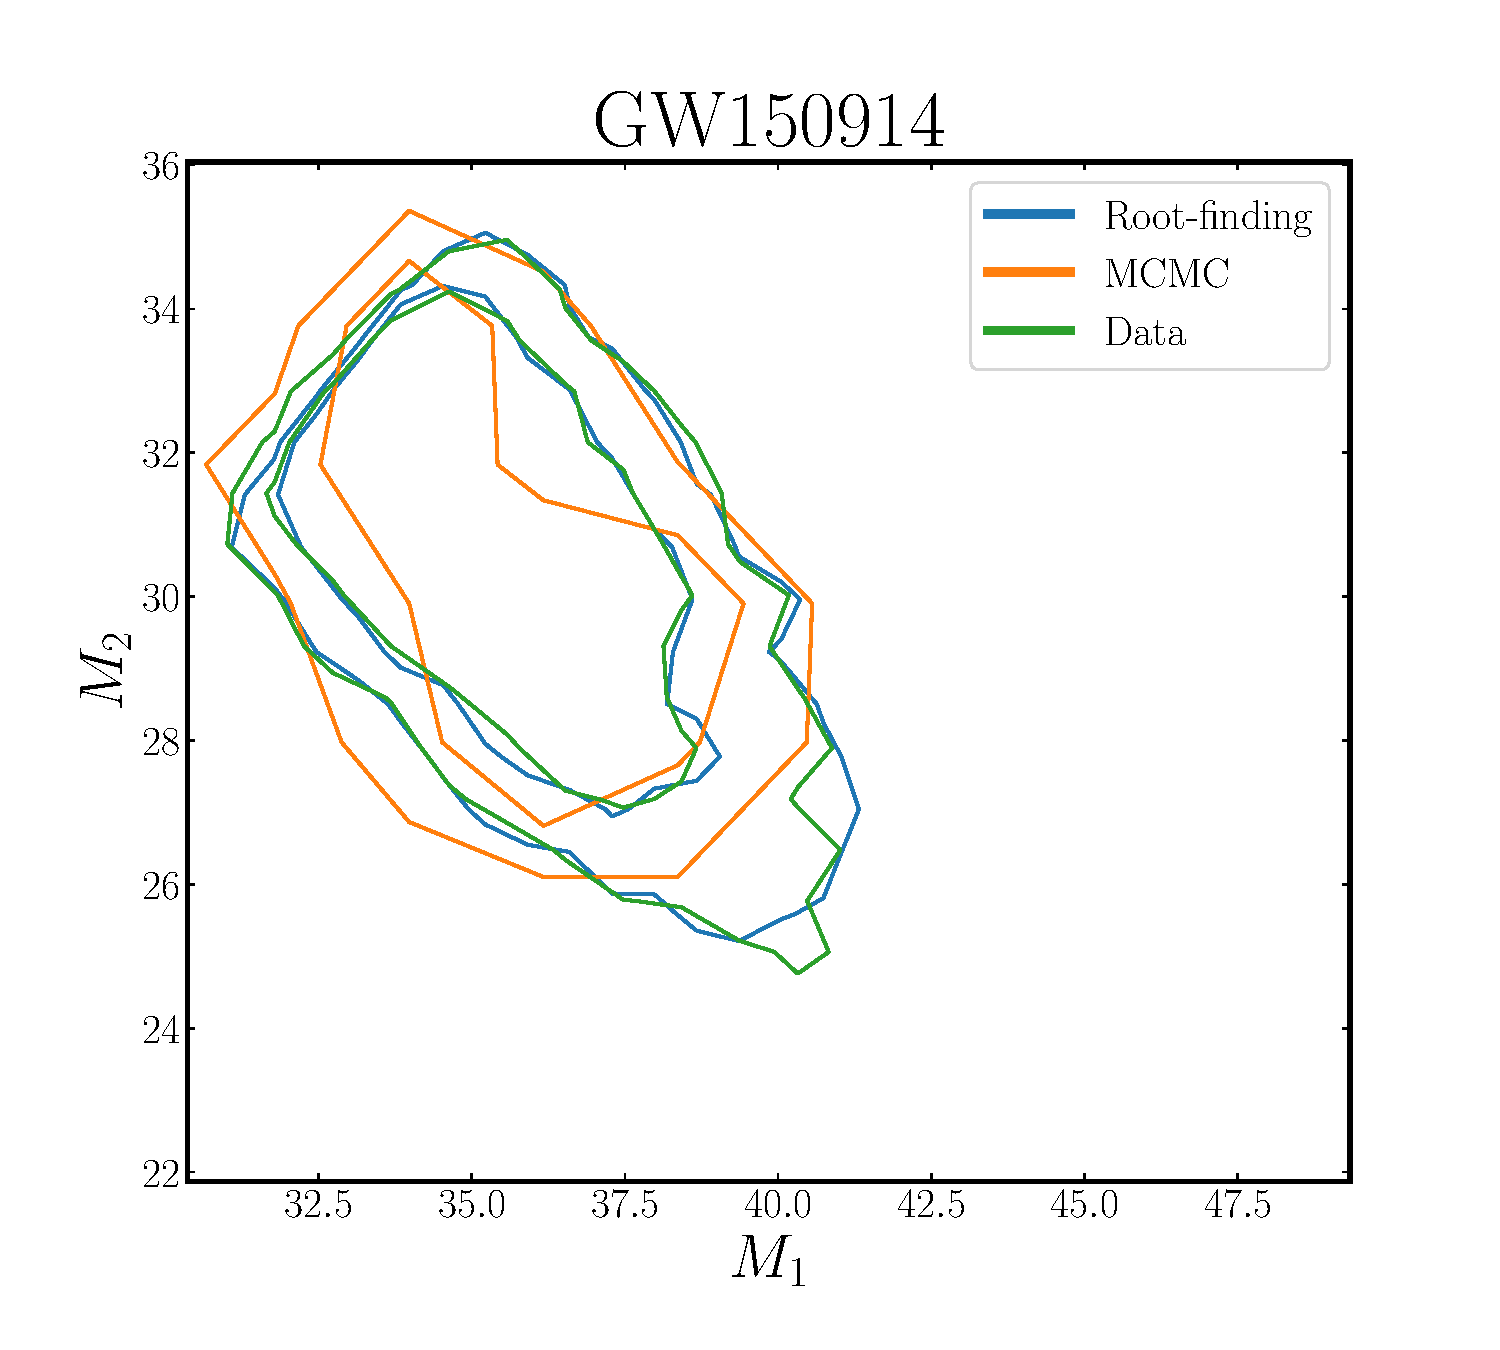
\includegraphics[width=0.49\textwidth]{figures/GW150914_reprojection.png}
% \caption{Caption}
% \label{fig:GW150914_reprojection}
% \end{figure}

\section{Discussion}

Interpretation:
\begin{enumerate}
\item Highlight the fact that we turn hyper-parameters into parameters.
\item Discuss this is need for high dimensional exploration.
\end{enumerate}



Caveats: 
\begin{enumerate}
\item Discuss events that cannot be complete transferred backward. From BSE angle and from LIGO posterior angle. Failure mode in mass.
\item We only assume BSE
\item Caveat on marginalizing over random samples.
\item Prior need to be applied after one translate the posterior, i.e. it is a post-processing step now.
\item How next generation "Progenitor synthesis" code should be built.
\item Rate
\item Failure studies go into appendix
\end{enumerate}

\end{document}
